%%%%%%%%%
\section{Modelling of top quark production}\label{sec:ttbar}
%%%%%%%%%

The backgrounds from \ttbar and single-top-quark production in both analysis channels are estimated from data-based correction factors in the normalization of the simulation.
A top-quark-enriched control sample is selected by applying all the analysis requirements except that the b-jet veto is inverted by requiring, instead, at least one b-tagged AK4 (or AK5) jet in the event.\\

For the $\ell\Pgn\qqbar$ channel, the comparison between data and simulation yields normalization correction factors for \ttbar and single-top-quark background processes evaluated in the pruned-jet-mass signal region
$65 < \mJ < 105\GeV$. The measured correction factors are 0.87 $\pm$ 0.04 and 0.83 $\pm$ 0.07 for the muon and electron channel, respectively, where the quoted uncertainty is only statistical.
The disagreement is consistent with the difference between NLO and NNLO shape prediction for large top quark \pt~\cite{Czakon:2015owf}.\\

For the $\ell\Pgn\bbbar$ channel, a unique correction factor is calculated with a simultaneous fit to number of data events in the muon and electron channels in the pruned-jet-mass region $40 < \mJ < 150\GeV$.
The difference in normalization between data and simulation is found to be 4.6 $\pm$ 5.6\%, where the quoted uncertainty is only statistical. \\

These scale factors include both the W boson signal and the combinatorial components mainly due to events where the extra b jet from the top quark decay is in the proximity of the W, and are used to correct the normalization
of the \ttbar and single-top-quark simulated background predictions in the signal regions. The relative uncertainties are used to quantify the uncertainty in the \ttbar and single-top-quark background normalization.

The \mJ distribution in the top-quark-enriched sample for the 13\TeV data $\ell\nu\qqbar$ analysis and for simulation is shown in Fig.~\ref{fig:tt-controlPlots13TeV_a}, while Fig.~\ref{fig:tt-controlPlots13TeV_b} shows the \nsubj distribution.
The same distribution is also shown for the $\ell\Pgn\bbbar$ analysis channel in Fig.~\ref{fig:tt-controlPlots8TeV}, where 8\TeV data and simulation are compared.
In all cases, the \mJ spectrum shows a clear peak for events with a W boson decaying to hadrons, including the combinatorial background, while a reasonable agreement between the shapes in data and simulation is observed.
Comparisons of data and simulation are also shown in Fig.~\ref{fig:tt-mtop8TeV} for other distributions such as the reconstructed \mlvj, as well as $m_\mathrm{top}^\mathrm{l}$ and $m_\mathrm{top}^\mathrm{h}$.
In the latter a clear peak at the top quark mass is visible.
%The distributions of the reconstructed $m_\mathrm{top}^\mathrm{l}$ and $m_\mathrm{top}^\mathrm{h}$ for the $\mu\Pgn$+H-jet channel are also shown in Fig.~\ref{fig:tt-mtop8TeV}, where the peak at the top quark mass is clearly visible.

\begin{figure}[!htb]
\centering
\subfigure[]{\label{fig:tt-controlPlots13TeV_a}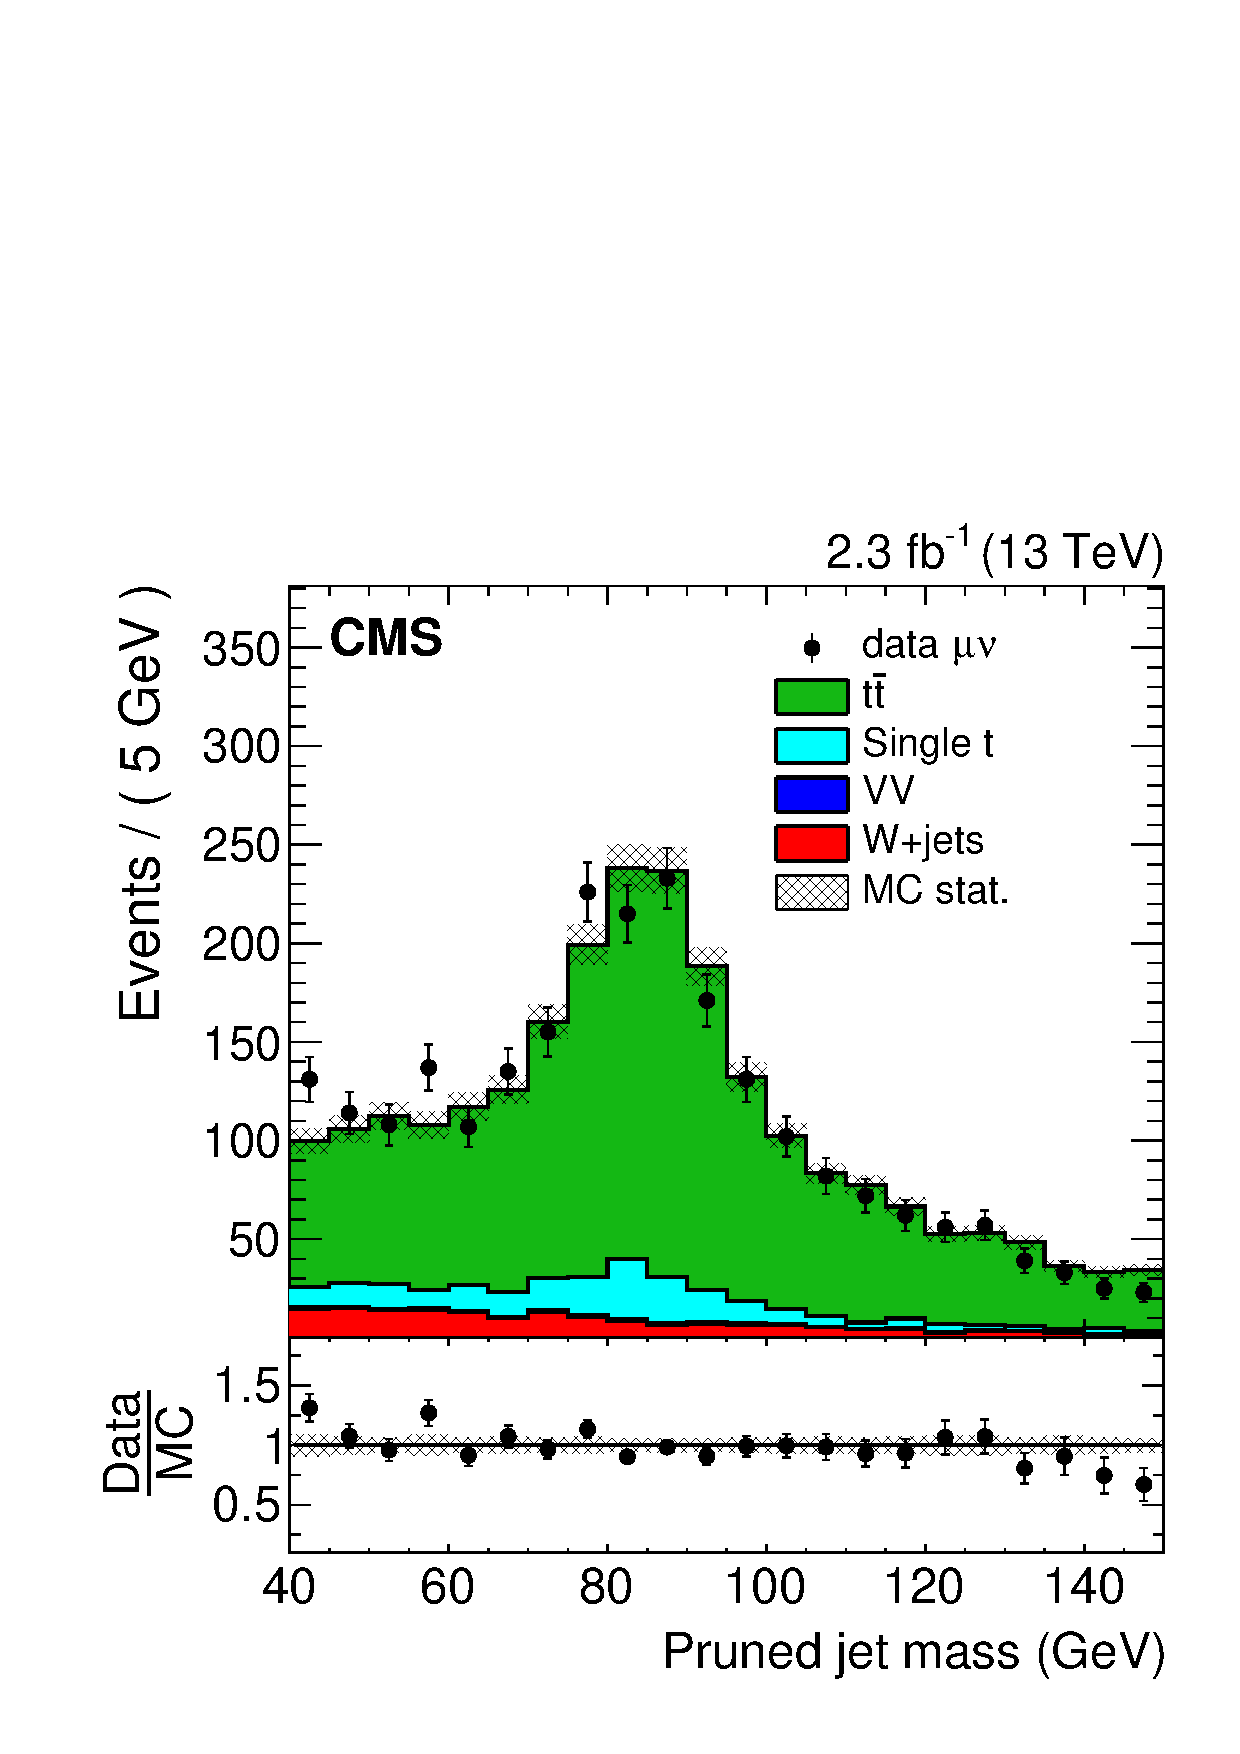
\includegraphics[width=0.45\textwidth]{\cheight/ttbar-pruned-jet-mass-mu-13TeV.pdf}}
\subfigure[]{\label{fig:tt-controlPlots13TeV_b}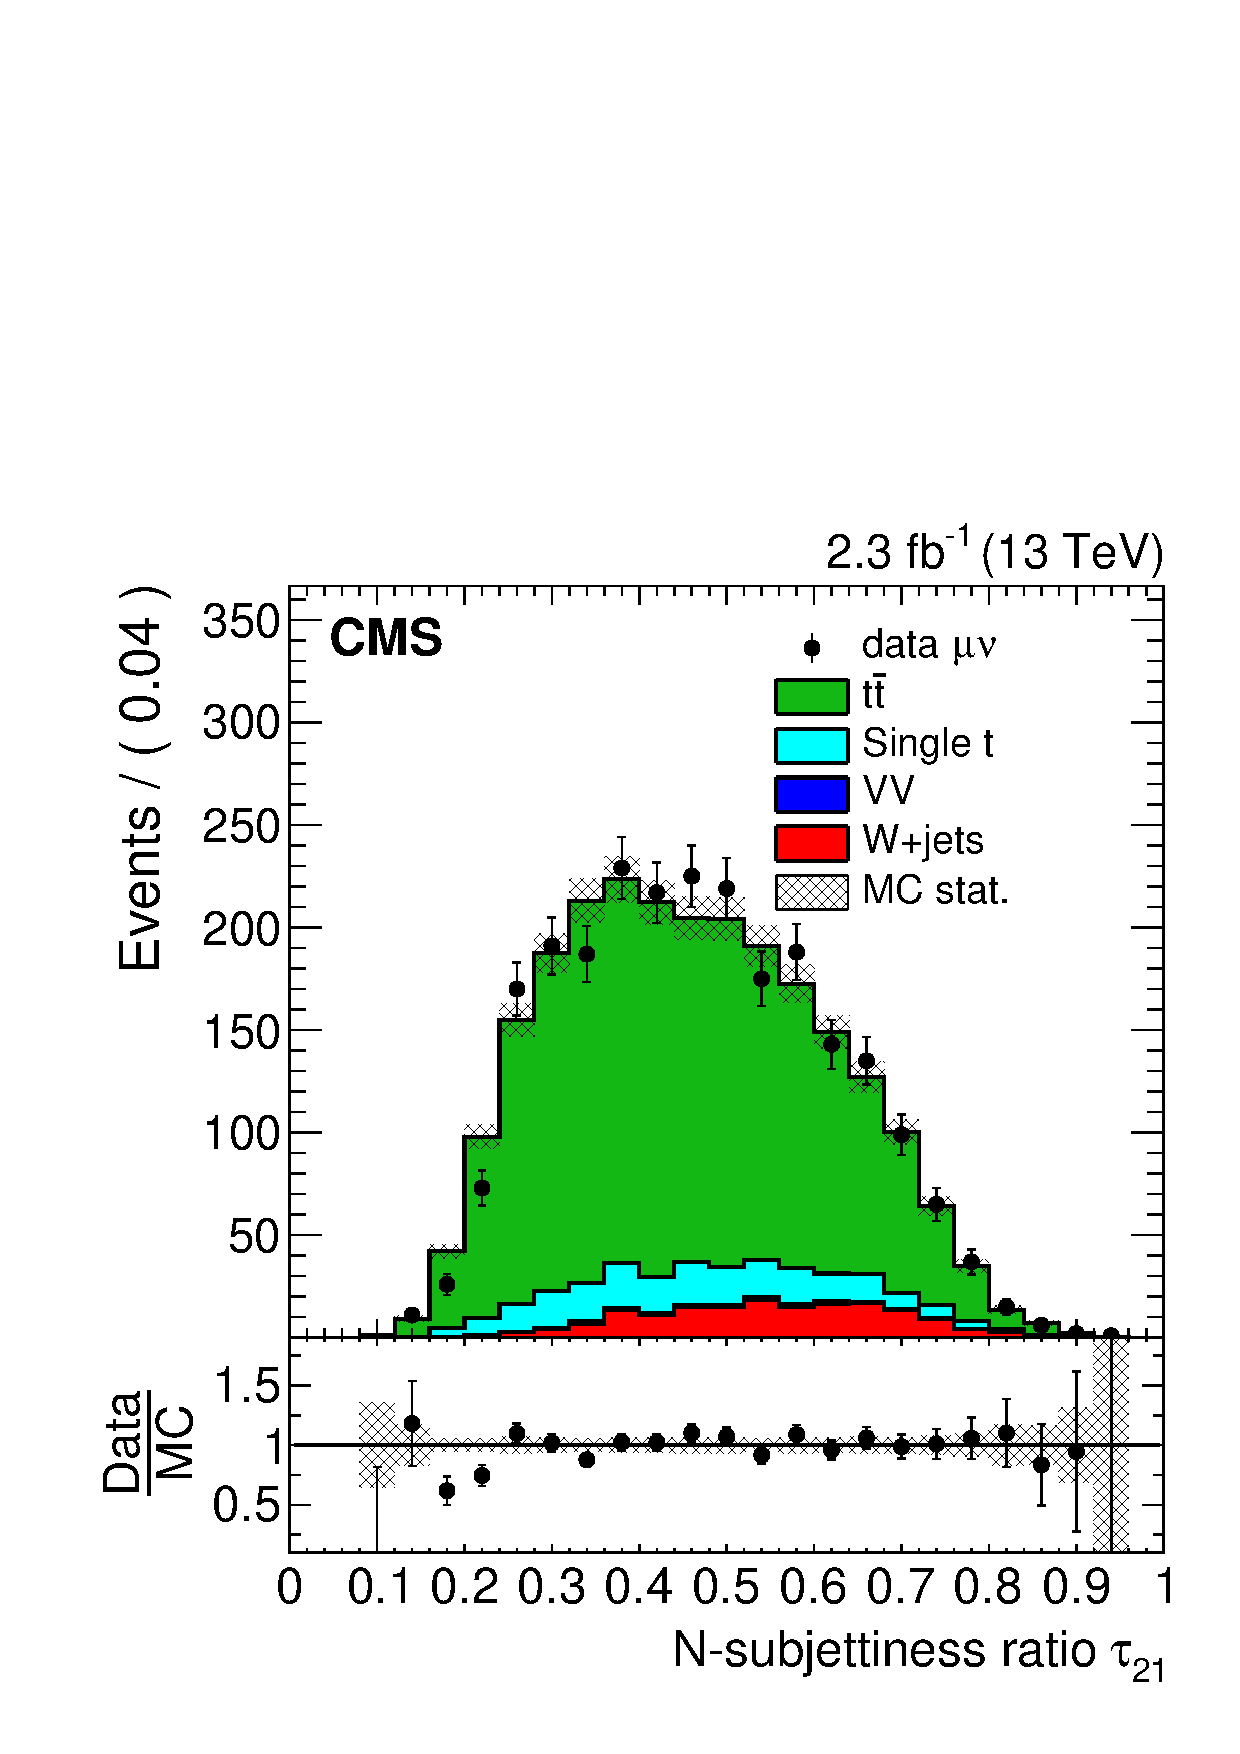
\includegraphics[width=0.45\textwidth]{\cheight/ttbar-tau21-mu-13TeV.pdf}}
\caption{Distributions in the N-subjettiness ratio \nsubj (a) and pruned-jet mass \mJ (b) from the top-quark-enriched control sample in the muon channel of the $\ell\nu\qqbar$ analysis. The \ttbar background is rescaled such that the total number of background events matches the number of events in 13\TeV data.}
\label{fig:tt-controlPlots13TeV}
\end{figure}

\begin{figure}[!htb]
\centering
\subfigure[]{\label{fig:tt-controlPlots8TeV_a}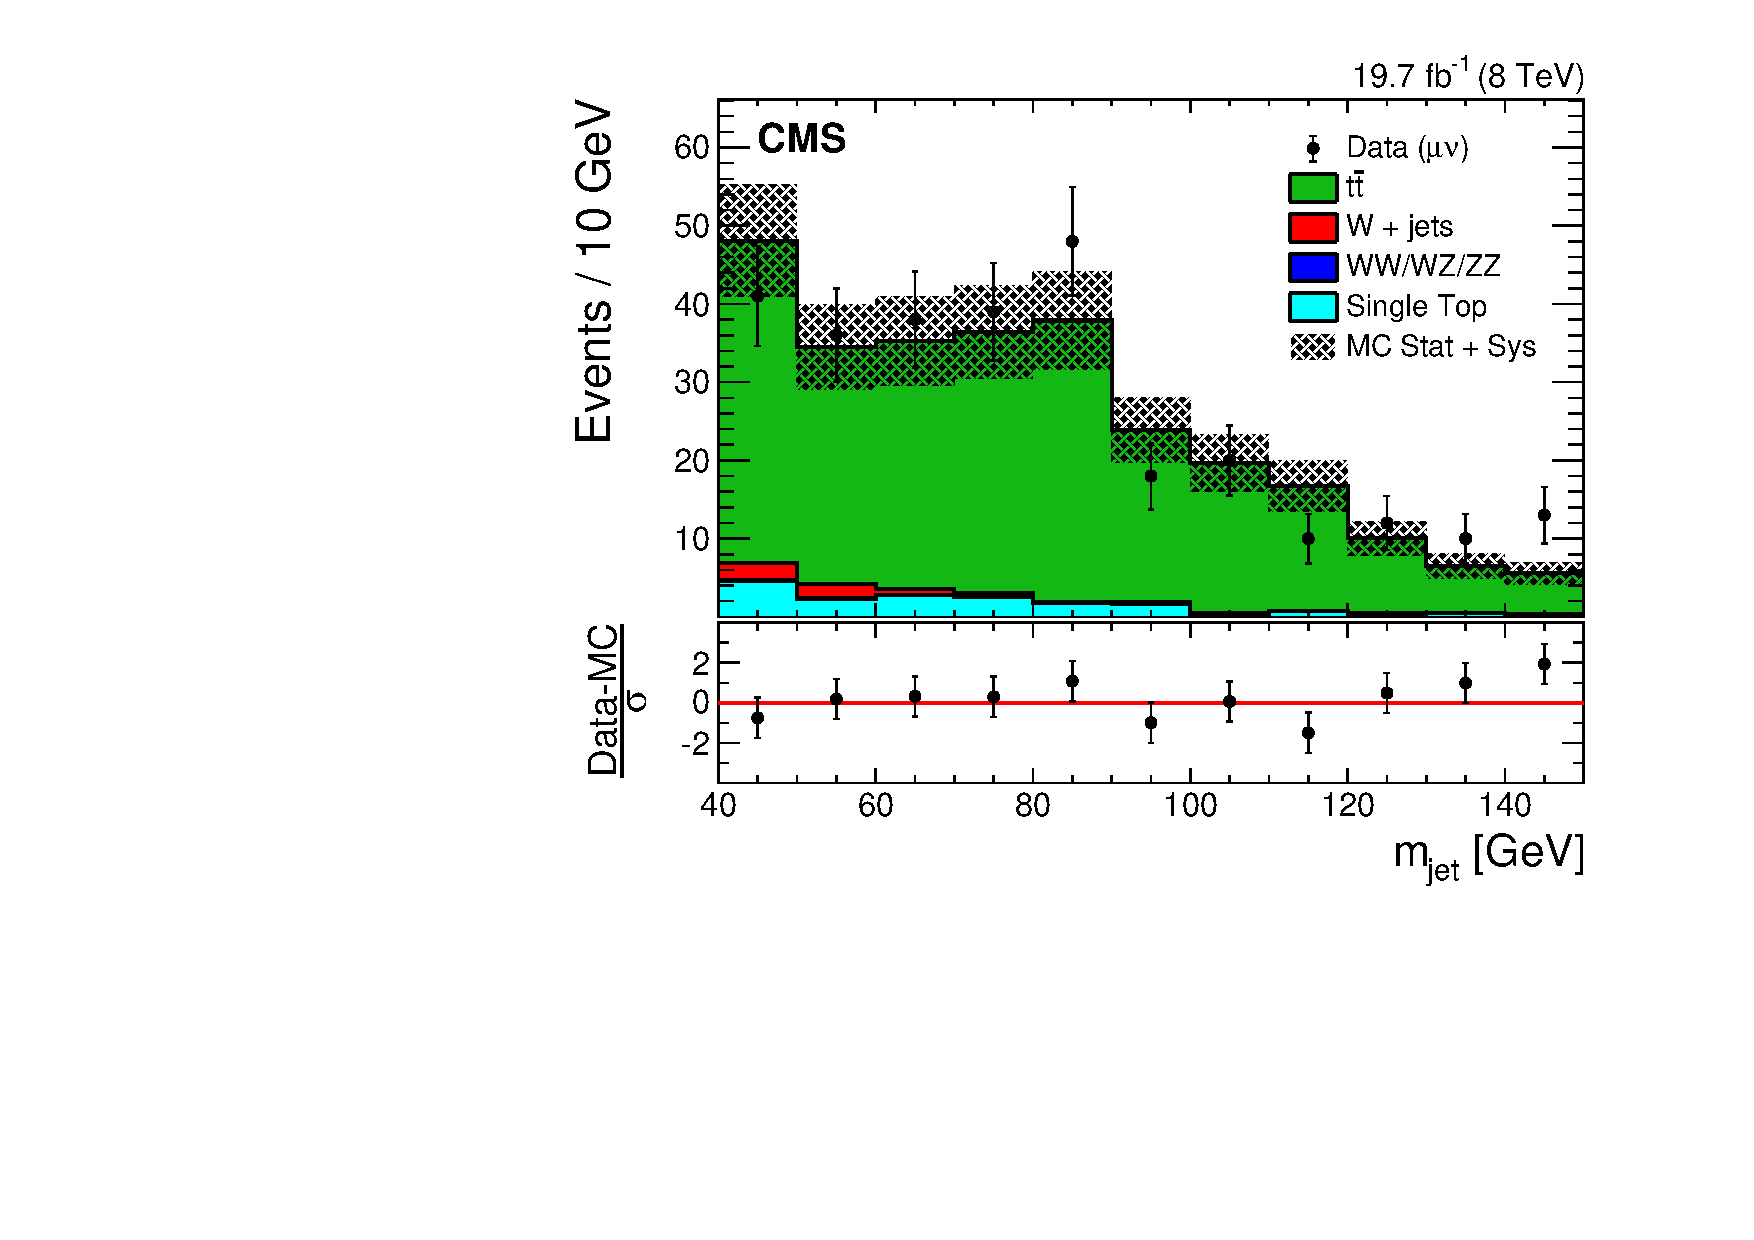
\includegraphics[width=0.45\textwidth]{\cheight/ttbar-pruned-jet-mass-mu-8TeV.pdf}}
\subfigure[]{\label{fig:tt-controlPlots8TeV_b}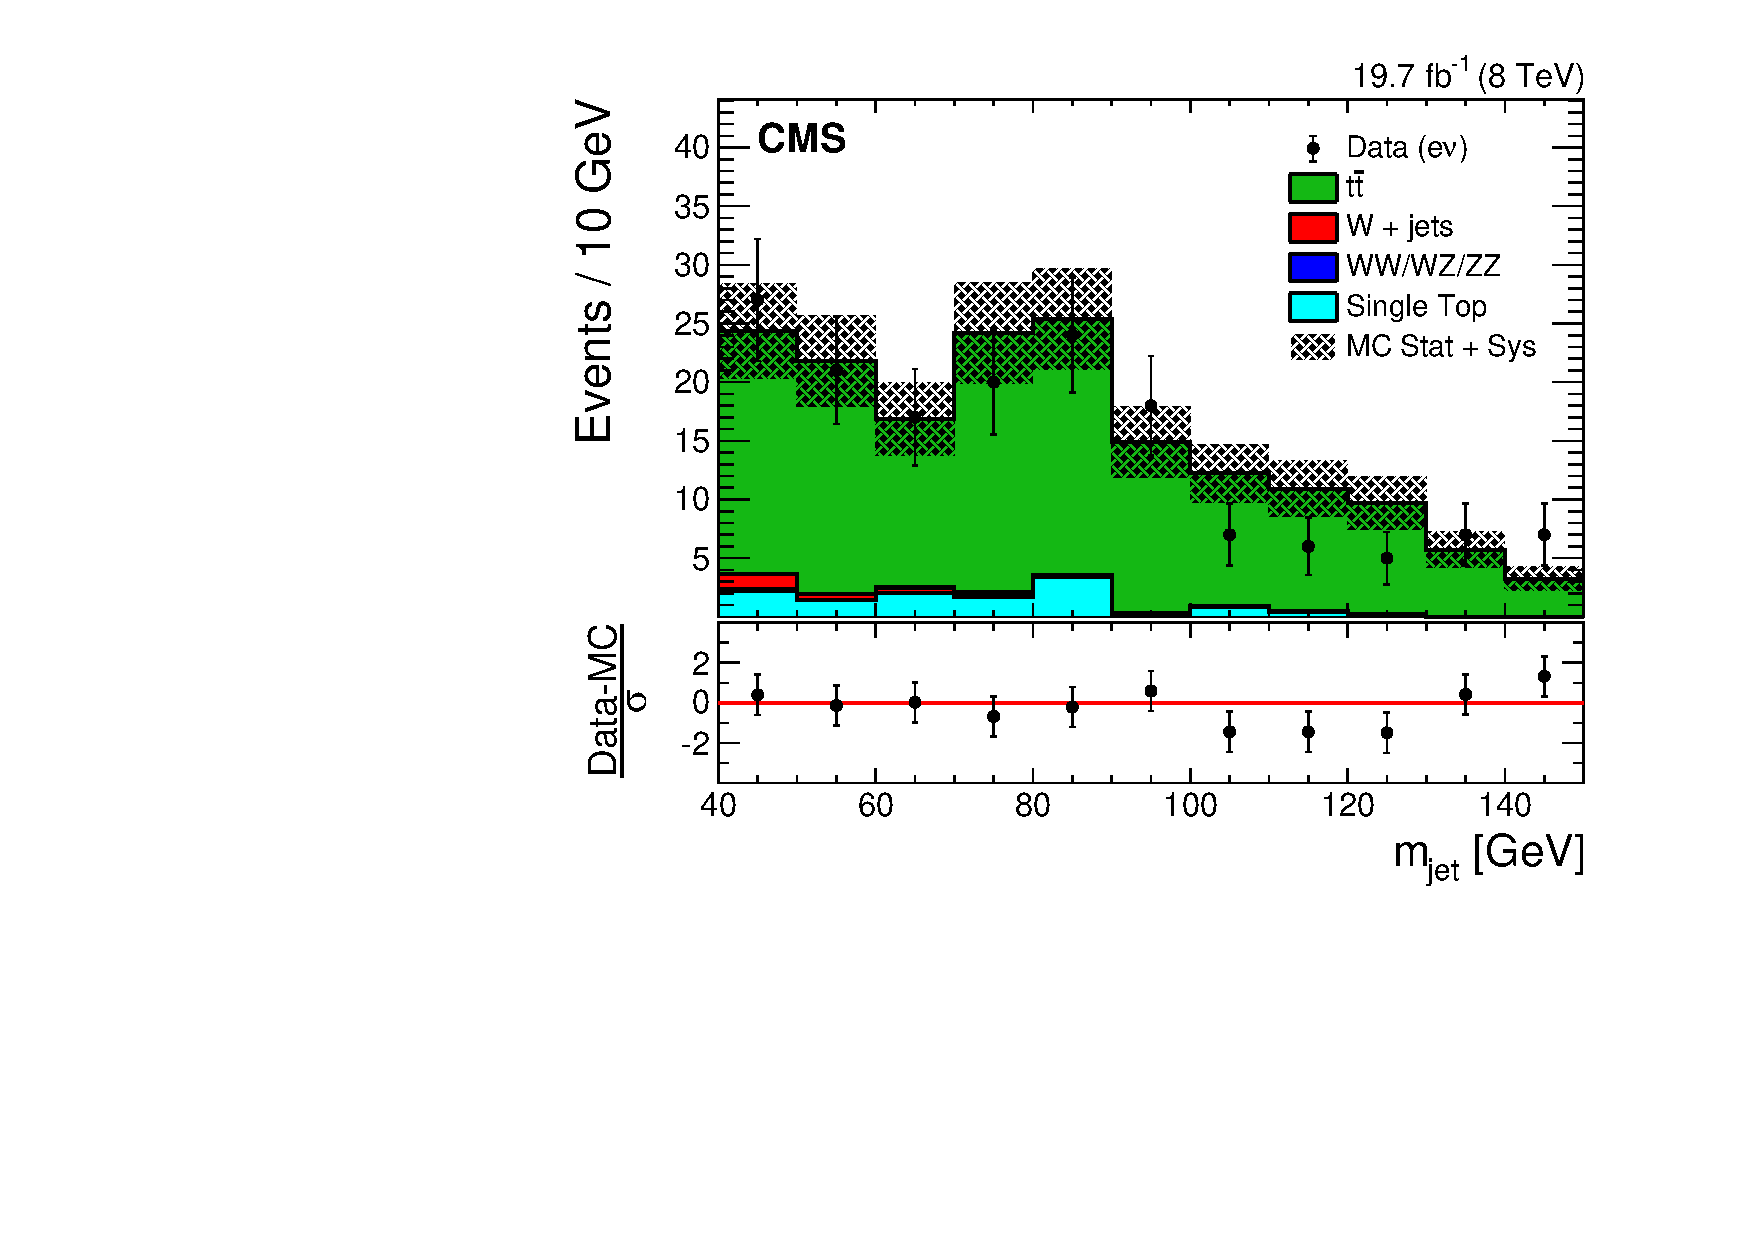
\includegraphics[width=0.45\textwidth]{\cheight/ttbar-pruned-jet-mass-e-8TeV.pdf}}
\caption{Distributions in pruned-jet mass \mJ in the top-quark-enriched control sample in the electron (a) and muon (b) channels of the $\ell\Pgn\bbbar$ analysis. The hatched region indicates the overall uncertainty in the background. In the lower panels, the bin-by-bin residuals, (Data - MC)/$\sigma$ are shown, where $\sigma$ is the sum in quadrature of the statistical uncertainty of the 8\TeV data, the simulation, and the systematic uncertainty in the \ttbar background.}
\label{fig:tt-controlPlots8TeV}
\end{figure}

\begin{figure}[!htb]
\centering
\subfigure[]{\label{fig:tt-mtop8TeV_a}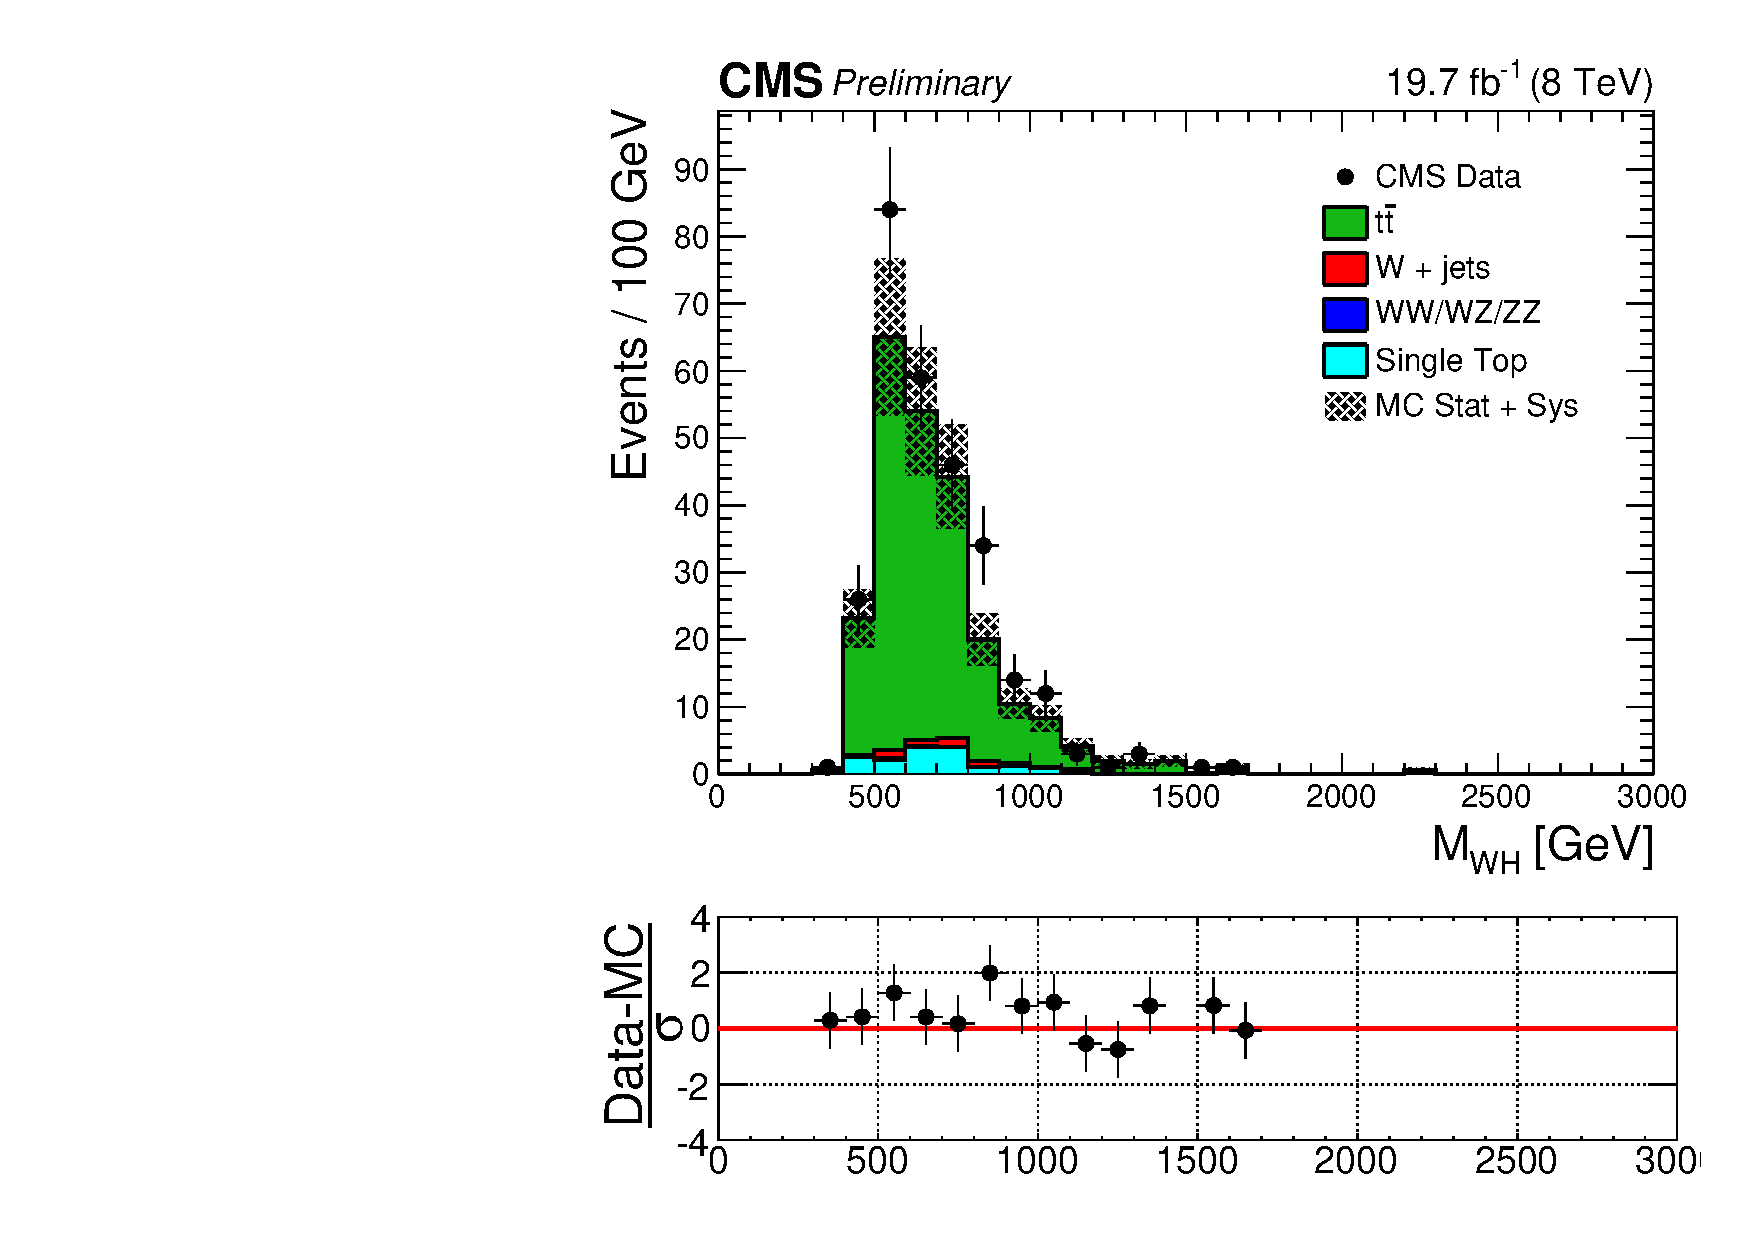
\includegraphics[width=0.45\textwidth]{\cheight/ttbar-dibosons-invmass-8TeV.pdf}}\\
\subfigure[]{\label{fig:tt-mtop8TeV_b}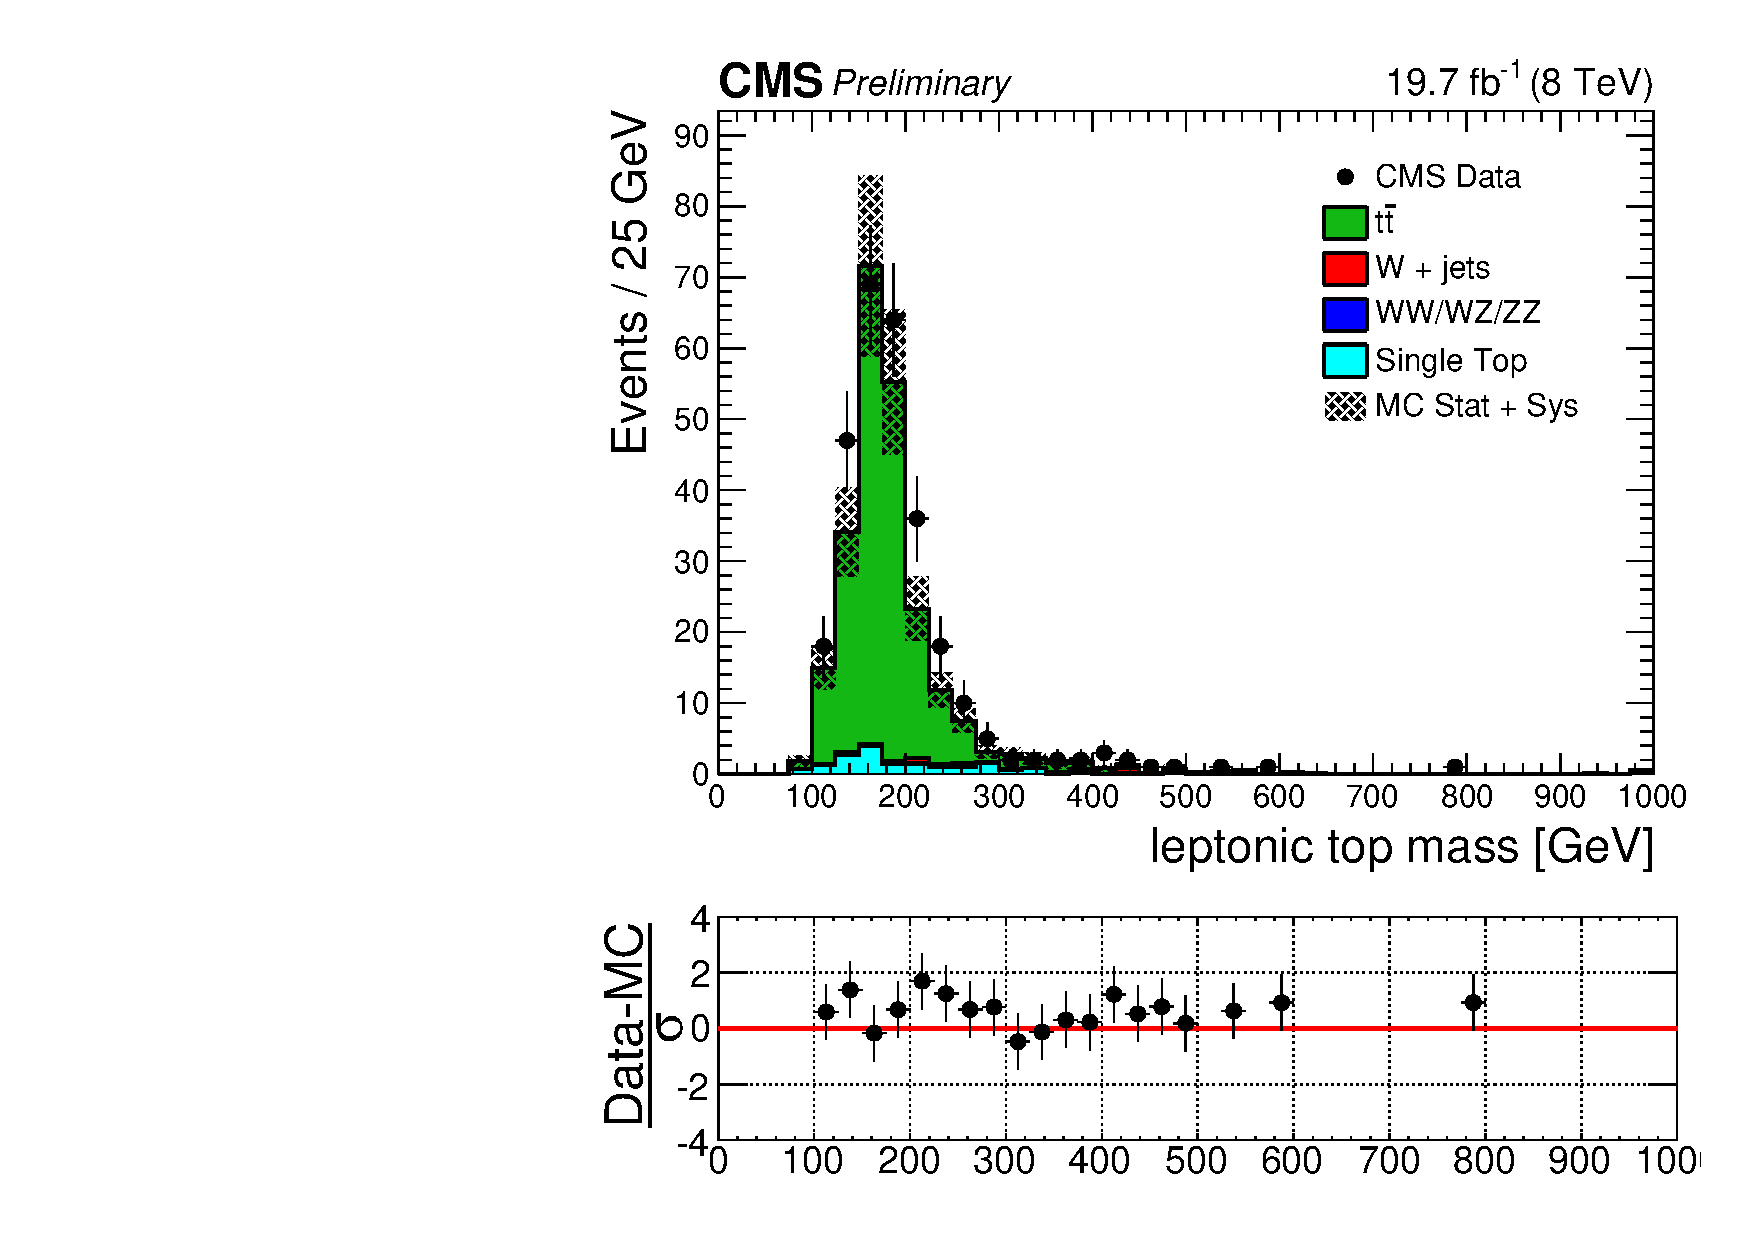
\includegraphics[width=0.45\textwidth]{\cheight/ttbar-mtoplept-mu-8TeV.pdf}}
\subfigure[]{\label{fig:tt-mtop8TeV_c}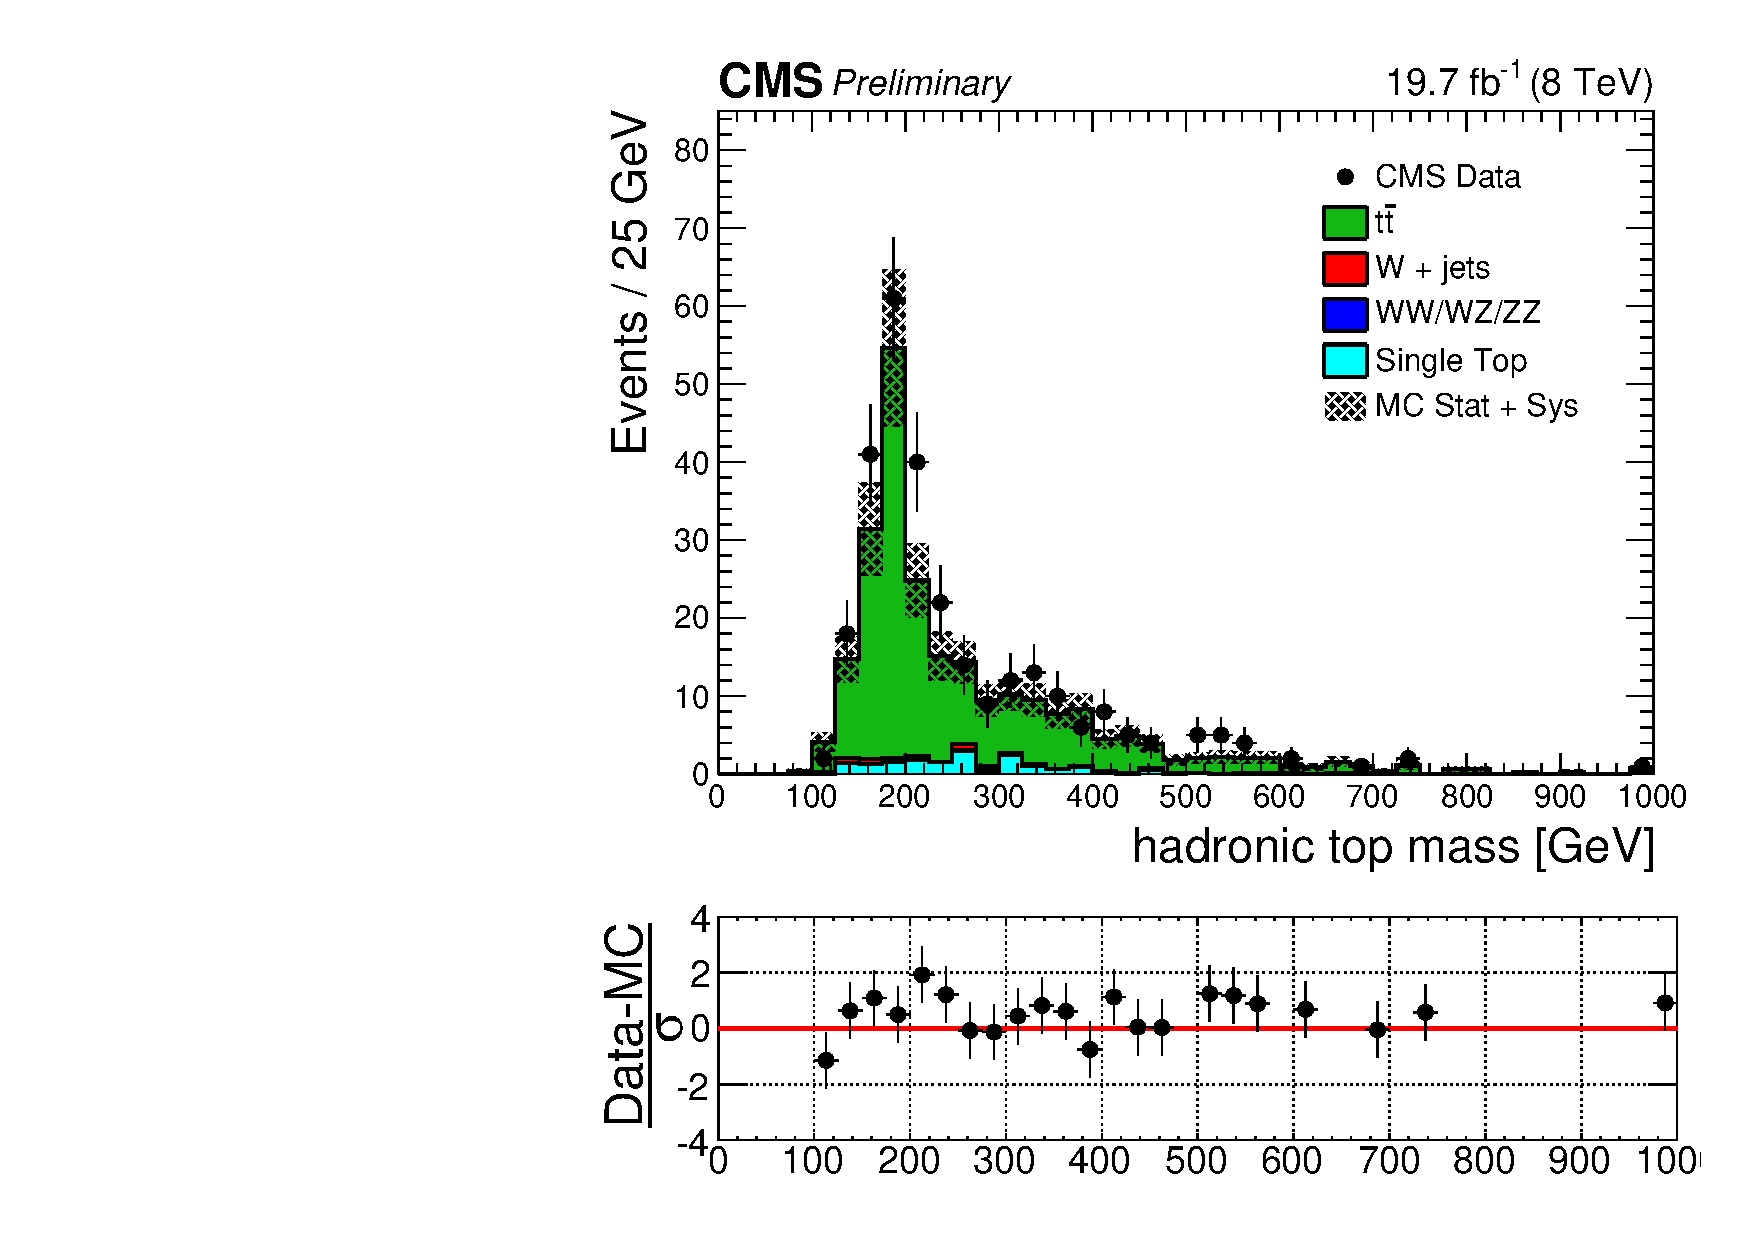
\includegraphics[width=0.45\textwidth]{\cheight/ttbar-mtophadr-mu-8TeV.pdf}}
\caption{Distributions for 8\TeV data and for simulation in \mWH (a), $m_\mathrm{top}^\mathrm{l}$ (b) and $m_\mathrm{top}^\mathrm{h}$ (c) in the top-quark-enriched control sample for the muon channel of the $\ell\Pgn\bbbar$ analysis.}
\label{fig:tt-mtop8TeV}
\end{figure}